

\chapter{Use of non linear optimization in MMVII}

\label{Chap:NLO}

This chapter is targeted for programmer that will increase MMVII, it mainly describe classes
interfaces in headers and a detailled example of using this classes in a cpp file.
 It's not usefull for advanced users; on the other hand,for programmer who will maintain the core of MMVII, 
more detailled documentation will have to be written.

At this step, the chapter may no theoreticall presentation, it assume that reader is familliar
with least square, linearization, Gauss-Newton, Schurr complements \dots


%---------------------------------------------
%---------------------------------------------
%---------------------------------------------

\section{Introduction}

%---------------------------------------------

\subsection{Quick formalization}

This chapter present the classes used in MMVII for non linear optimisation using some Gauss-Newton methods. 
By non linear optimisation, we means minimize $F(X)$ with :

\begin{equation}
      F(X) = \sum_{j=1,M} w_j f_j(X)^2  \;  X \in \RR^n  \label{EqNLOInit}
\end{equation}

The assumpution on the problem are classical :

\begin{itemize}
   \item we have an initial guess $X_0$ on $X_{min}$  , this guess is sufficiently 
         good for the local minimal we will (hopefully) find to be a global minimum;

   \item the function $f_j$ are differentiable (some weaker hypothesi are also possible)

\end{itemize}

The service offered by MMVII are typically those a Gauss-Newton iterations : 
use current estimation $\tilde X$ of $X_min$ for linearizing the $f_j$ and 
solve equation $\ref{EqNLOInit}$ by least square methods.

%---------------------------------------------

\subsection{2d-Triangularton problem in general}

We will illustrate the presentation by a detailled example that is used for testing correctness of the
implementation. Also relatively basic, this example should be sufficient for a first 
understanding and utilisation of the MMVII classes. The $2d$-triangulation problem we treat
here is the following :

\begin{itemize}
    \item we have a set of points $P_1 \dots P_n$ , each $P_k$ belongs to $\RR^2$;

    \item we ignorate the exact values of $P_k$ but we have an initial estimation  $P^0_k$
          which is not too bad, whatever it means;

    \item for a certain number of pair $P_i,P_j$ we have a measurement of the distance $d_{ij}$ between
          $P_i$ and $P_j$,
\end{itemize}

The triangulation problem  consist to use the measurement of distances for recovering the unknown
value on $P_i$.  Let $M$ be the  number of pair for which we have measurement 
Let $X \in \RR^{2n} = \{P_1 \dots P_n\}$ be the unkown vector,
we typically want to find $X$ that minmize $D$ defined by :

\begin{equation}
      D(X) = \sum_{j=1,M} (d_{ij} -d(P_i-P_j))^2  \label{EqConsDist}
\end{equation}


Of course as the fonction $D$ is invariant to any isometry of the plane, the minimization
of $D$ would be an ill-posed problem, as for any set of points, its image by a global rotation
will give the same value. To ensure uniqueness of the solution  will force the value of
a certain number of coordinates.

%---------------------------------------------

\subsection{2d-Triangularion in this example}

As we want the example to be as simple as possible, and also we want to use it for checking
the correctness, the data will be different from a real one , the figure~\ref{fig:NetFull} illustrates 
this network:

\begin{itemize}
    \item the "real" value of points will be positionned on a regular grid, typically we
           will have $(2*N+1)^2$ points, each point having integers corrdinate 
           $(x,y) \in [-N,N]^2$

    \item we will have measure between pair of point that  are $8$-neighoor i.e
          $max(|x-x'|,|y-y'|)\leq 1 $ , this is sufficient for the solution to be unique
          up a rotation ;

    \item in real life  $d_{ij}$ would be noisy, but here in this simulation example we
          use the exact value because, to check correctness of the library, we want to check 
          that we are able to recover the exact values of coordinates.
\end{itemize}

Regarding the arbirtrary constraint we will keep it as simple as possible, so 
considering the two points of the grid  $A=(0,0)$ and $B=(0,1)$ , we will add the following
constraint to the minimization :

\begin{equation}
      x_A=0  \;  y_A=0  \;  x_B=0 \label{Eq:FixVarAB}
\end{equation}

The two first constraint freeze the solution in translation, while the last one freeze the rotation.


\begin{figure}
\centering
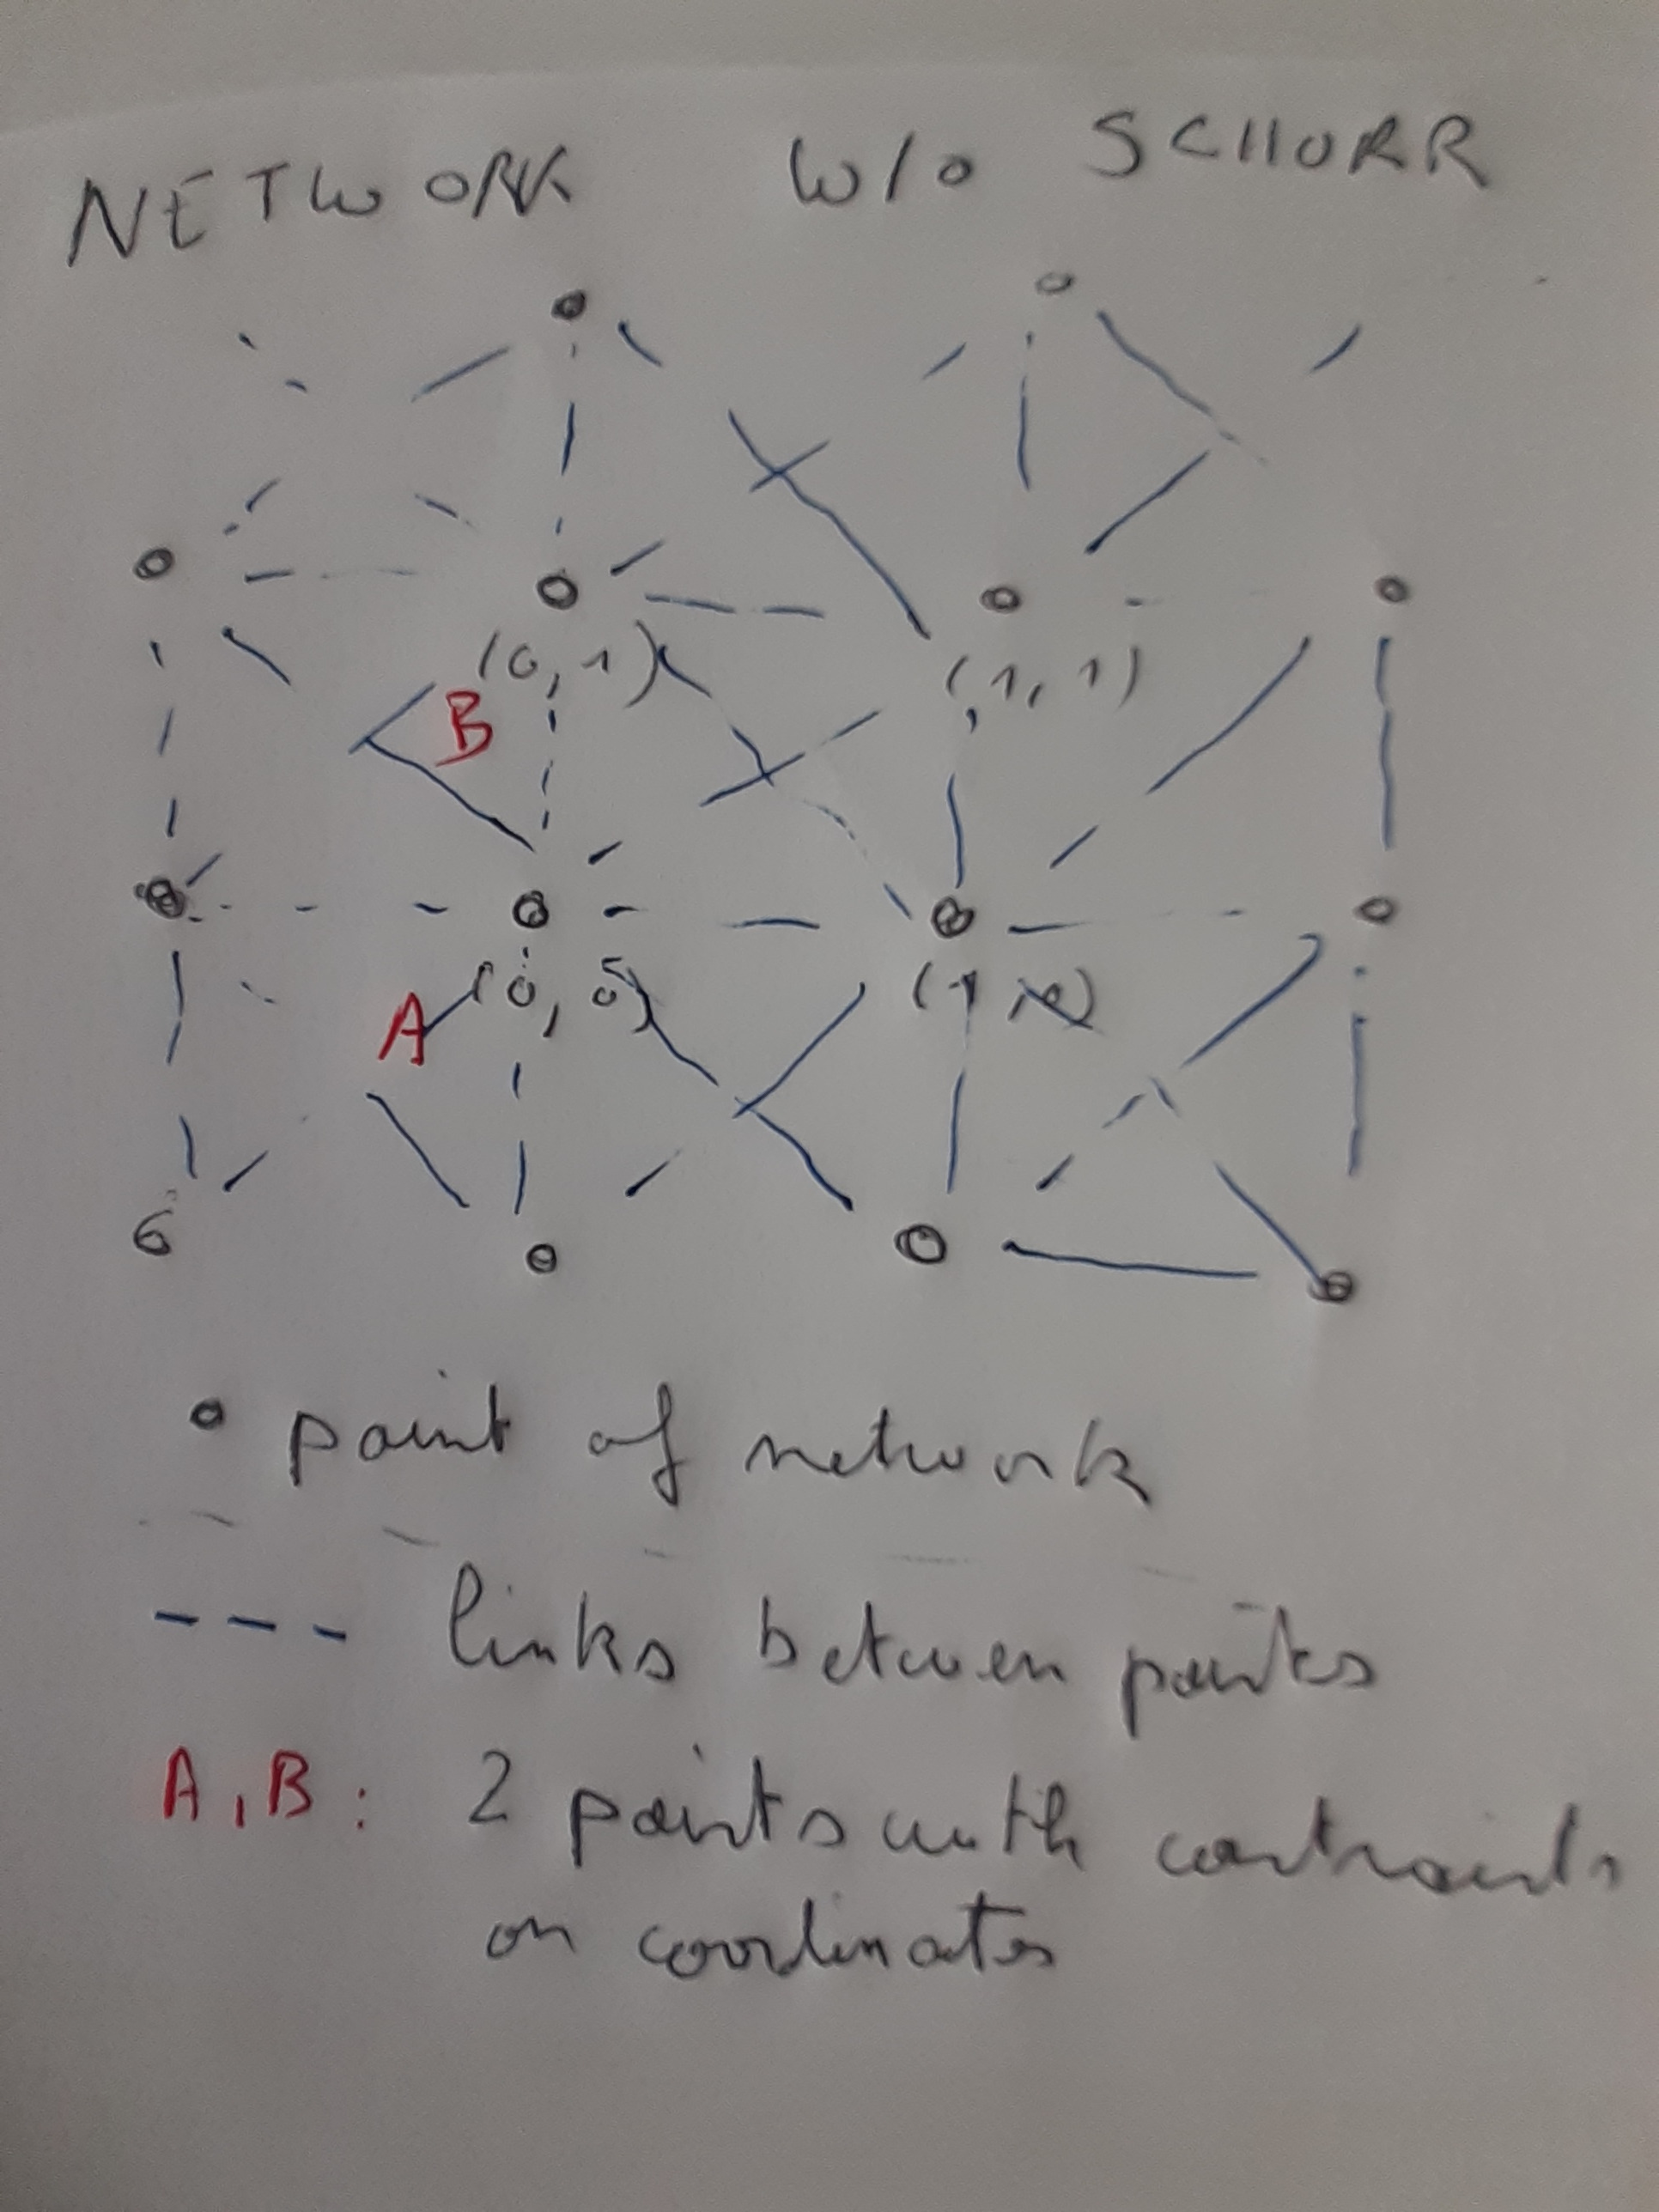
\includegraphics[width=12cm]{Methods/Images/T90-NetFull.JPG}\caption{Network, case w/o schurr}\label{fig:NetFull}
\end{figure}



%---------------------------------------------

\subsection{Use of schurr complement}

Schurr complement is an efficient way to treat the case where there is a subset of variable that 
occurs in \ref{EqNLOInit}, but for which we are not specially interested in exact values ,
 however but we want to take them into account rigourously in 
the computation of the others. Once we know
\emph{all} the equations where such  subset of variable is involved, schurr
complement offer a way to eliminate them without altering the value of the minimum.

A typicall case is in bundle adjsutment, when we are interested only to the value
of camera parameters and not by the value of $3d$ points involved by the projection
equation. In this case, suppose we will typically  have $1000$ camera and $1000000$ points,
doing schurr elimination can reduce the system from $3000000$ unkwnon to $6000$.


In our toy example, the schurr complement will be purely artificiall. When the
{\tt WithSchurr}  option is activated, the network is modified in the following
way , the figure~\ref{fig:NetSchurr} illustrates 

\begin{itemize}
    \item all the points on the line $x=1$ are considered as temporay variable,
          i.e variable that we want to eliminate, we will not  know their value at the
          end of the computation; 

    \item there will be no conexion between points of line $x=1$ (for example $(1,2)$
          and $(1,3)$ that were connected in previous case are non longer
\end{itemize}

\begin{figure}
\centering
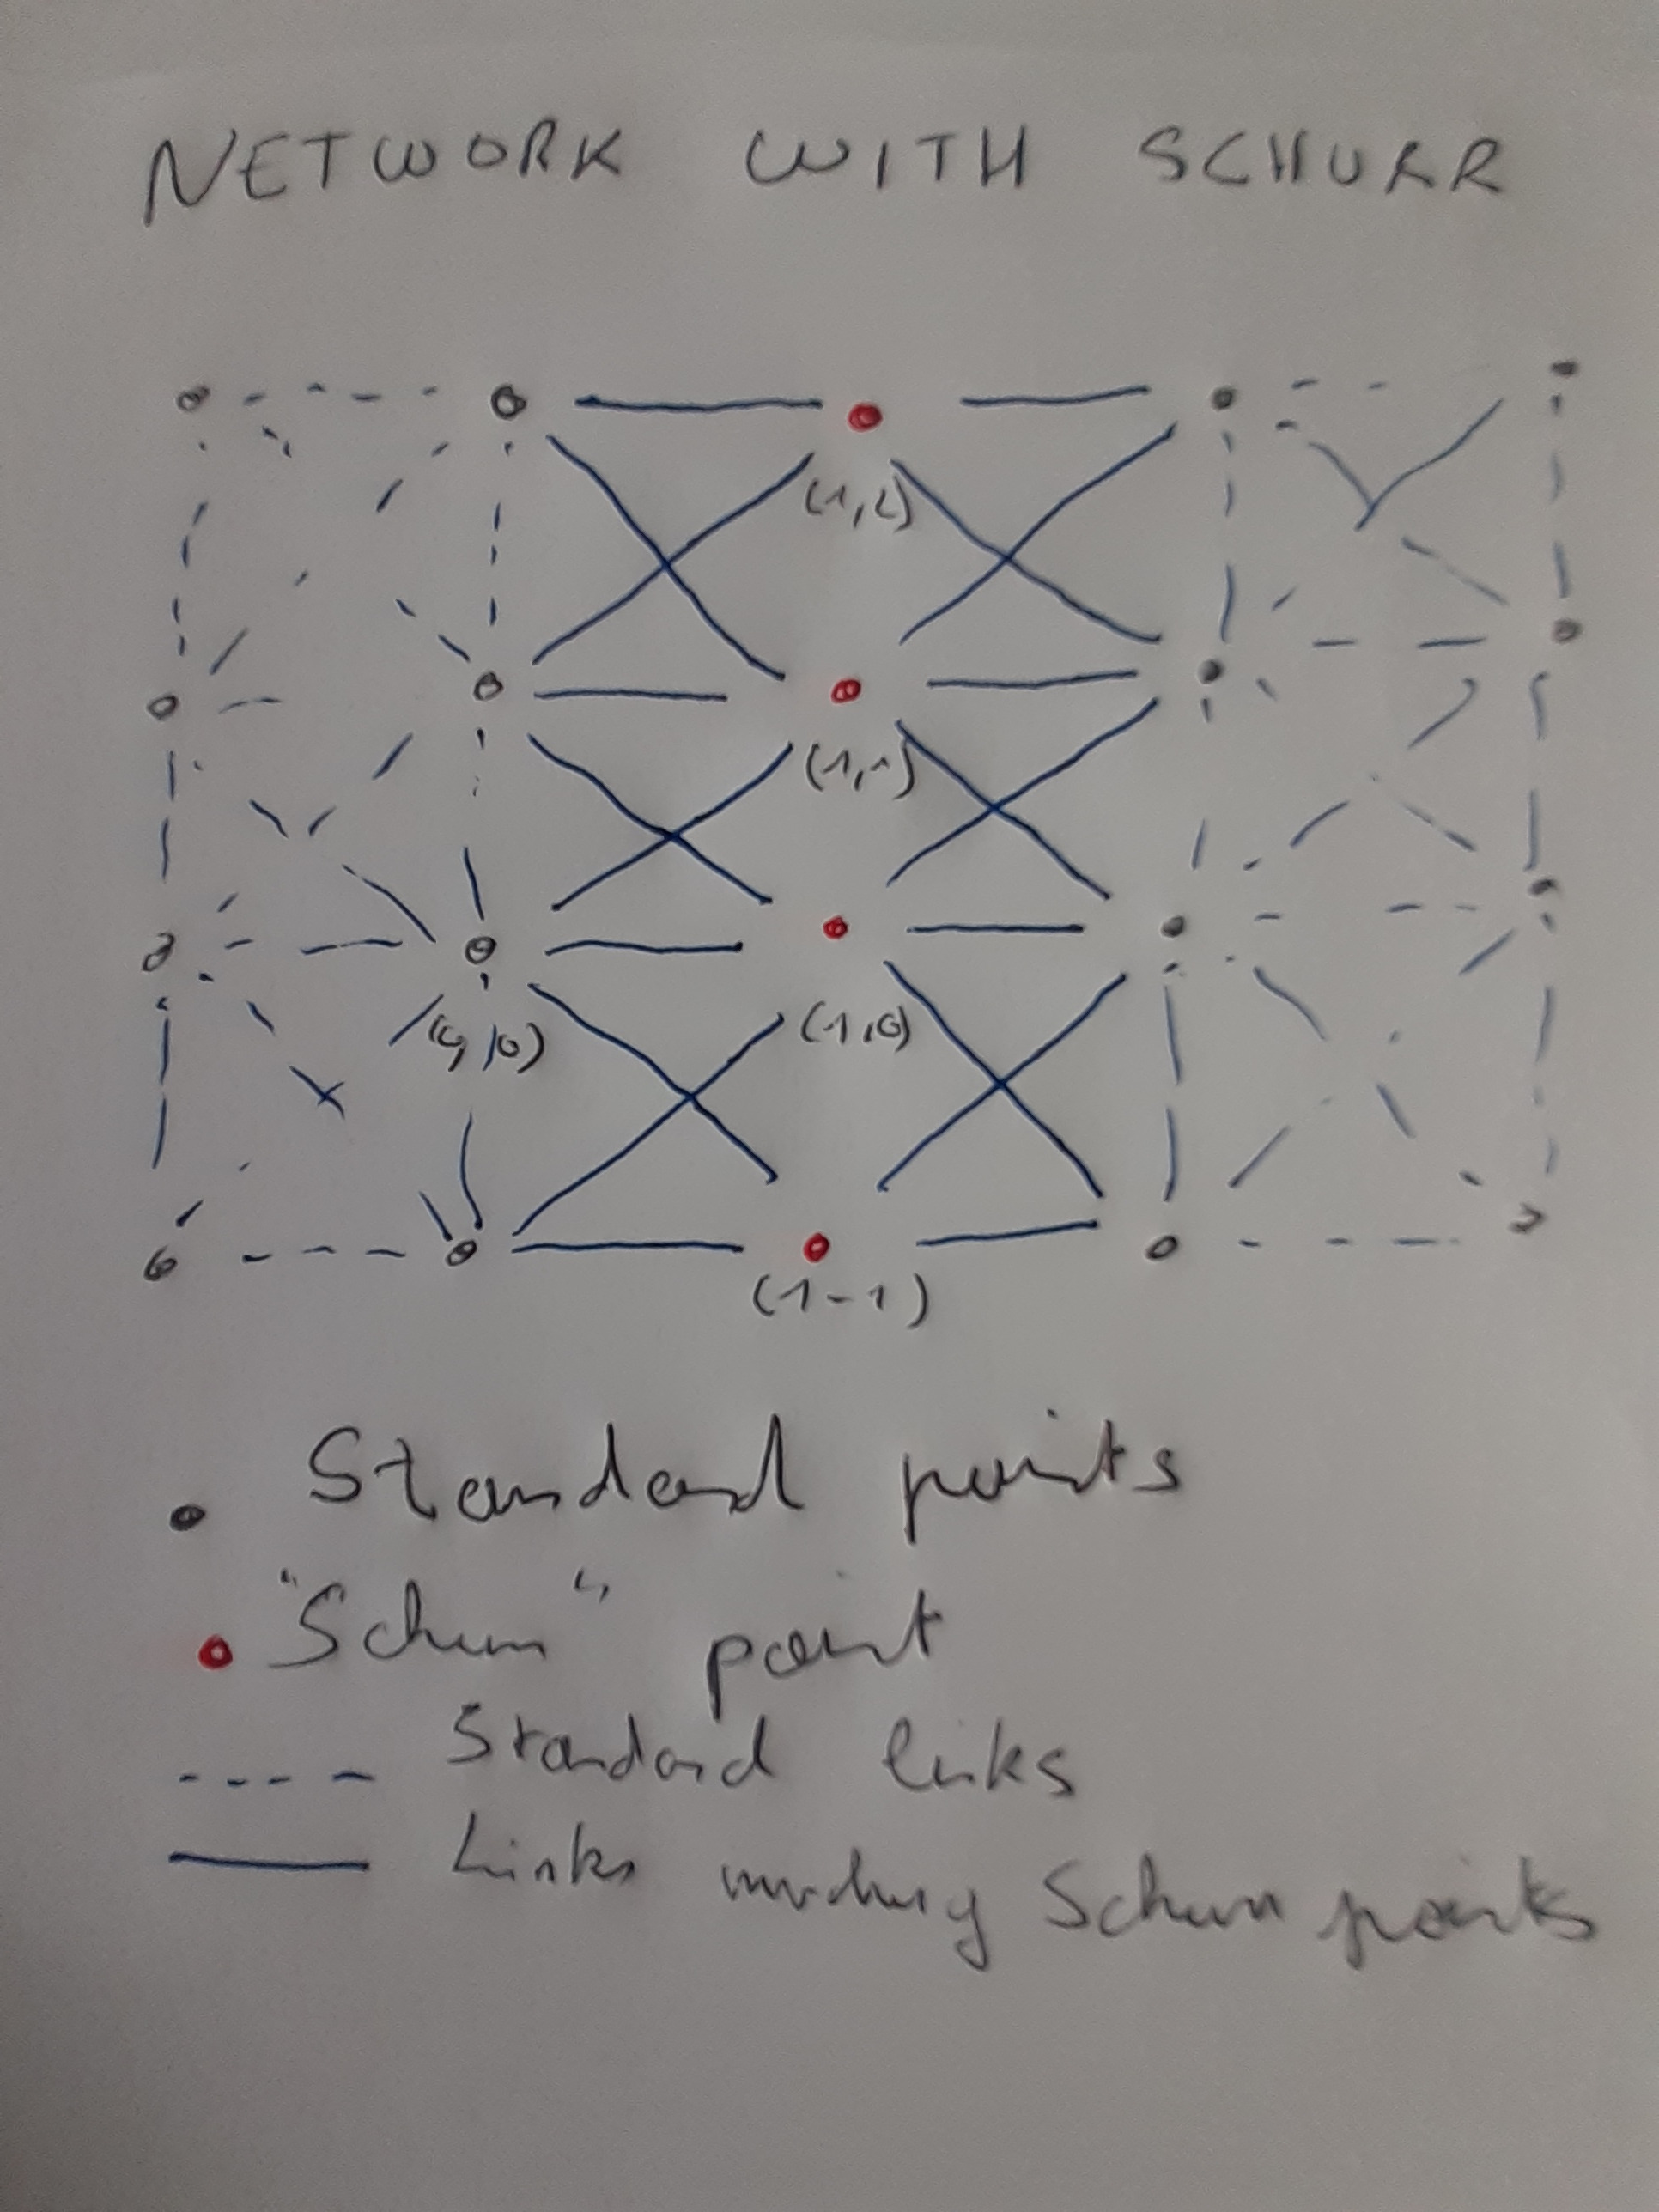
\includegraphics[width=12cm]{Methods/Images/T90-NetSchurr.JPG}\caption{Network, case with schurr}\label{fig:NetSchurr}
\end{figure}

%---------------------------------------------

\subsection{Files of MMVII involved}

We make a quick enumeration of files of MMVII that are to access for understanding :

\begin{itemize}
    \item {\tt include/MMVII\_SysSurR.h} contains the declaration of the class relatives to
          non linear optimisation, from the user point of view the main class
          is {\tt  cResolSysNonLinear};

    \item {\tt src/Bench/BenchResolSysNonLinear.cpp} contains the code for the $2d$-triangulation
          example;

    \item {\tt src/SymbDerGen/Formulas\_Geom2D.h } and {\tt src/SymbDerGen/GenerateCodes.cpp } 
          contains the code for generating the automatic differentiation 

    \item {\tt src/GeneratedCodes/CodeGen\_cDist2DConsVal.cpp } contains the code for 
          generating the automatic differentiation , also it is theoretically not necessary 
          to see it for using it, it's no harm to be curious and not use it as a black box;
          by the way in real case use, it will not be necessary to look at the code that you
          will generate.
\end{itemize}

%---------------------------------------------
%---------------------------------------------
%---------------------------------------------

\section{Computing functions and their derivatives}
\label{Compute:Deriv:SysNL}

%---------------------------------------------
\subsection{Motivation}

For Gauss Newton iteration, in equation \ref{EqNLOInit}, we will need to compute not only
the $f_j$ but also all its partial derivative $\frac{\partial f_j}{\partial x_i}$
relatively to all variable $x_i$ used in $f_j$.  There are many way to do it,
and to be honest  all have  pro and cons :

\begin{itemize}
    \item numerical derivative are the most simple, but they are slow, and can be unacurrate
          when the "small" value are not correctly choosen;

    \item hand crafted derivative are accurate and can be fast, however they can be complicated
          to write for real case formula (like arrise in bundled adjustement) and can be
          a nightmare to maintain when a "small" change occurs in the formulas;

    \item jet derivative, like used it Ceres, are almost as simple to use as numericall, once
          you have the library,  and much faster and accurate as numericall ones; they are much
          easier to use and maintain as  hand crafted ones, but can be also slower than
          handcrafted;

    \item symbolic derivative and code generation, can be a bit more complicated to use
          than jet, especially the first time; however after  this quick learning step
          they are as easy as jets to use,  easy to maintain and, in some case, much
          faster.
\end{itemize}

The solution implemenented in MMVII in based on symbolic derivative with code generation.
This choice was made because it is believed that programmer that will goes into the
core of MMVII have rather high requirement in code efficiency and are ready to pay a
small learning steps.

%---------------------------------------------
%\section{Generating the code}

          %  - - - - - - - - - - - - - - - - - - - 

\subsection{class for specifying the formulas}

In this  example, we have only one formula we need to compute and derivate, it's
the formula of equation~\ref{EqConsDist}.  First introduce a bit of MMVII's jargon  :

\begin{itemize}
   \item in this formula we have two different kind of variables the $P_i$ and $P_j$
         and the $d_{ij}$;
         
   \item for the $P_i$ themselves we have no direct observation , we only have initial value,
         and our target is precisely to compute their values; they will be named {\tt unkowns};

   \item for the $d_{ij}$ we know their values (it could be with some uncertaincy, but that'
         another story) and dont try to compute it, they will be name {\tt observations}.
\end{itemize}

The class {\tt cDist2DConservation} in file  {\tt src/SymbDerGen/Formulas\_Geom2D.h } contains
all the information that are required for generating code. It must define $5$ members :

\begin{itemize}
   \item a contructor, that does nothing for such a basic example

   \item a method {\tt VNamesUnknowns} that return the vector of names of unkown ,
         here we have $2$ points and $2$ coordinates $x,y$ for each points so the
         vector has a length of $4$;  the names will be used for code generation;

   \item a method {\tt VNamesObs} that return the vector of names of observations ,
         here we have a single observation which is the targeted distance between 
         $P_1$ and $P_2$;  the names will be used for code generation;

   \item a method {\tt FormulaName}  that return the name of the formula itself,
         the method will be used for the name of class and files containing the generated
          code;

   \item a method {\tt formula}  this is the core of the class, this method
         take as input a vector of unknown and a vector of observation and return
         a vector that is the result of the  computation  (typically a residual
         when used in context of gauss newton);  the type of {\tt tUk} of the
         i/o vectors and of temporary variable, is not very important at this step,
         it's suffice to know that it is a type on which most current mathematicall
         operation are defined (and can be completed when missing), they represent
         mathematicall formula as symbolic tree; see \RefFantome for detailled
         explanation on the type {\tt cFormula<Type>} defined in 

\end{itemize}

Regarding the $3$ methods that  return names, as they are used as \CPP identifier
its important that they contains only valid character (alpha numeric and {\tt\_} ,
no {\tt + - ...}),  also it's important that  inside a vector they are unique.
Apart of that, their exact name is unimportant, but giving names semantically
meaningfull is usefull if a human want to read the generated code (something we
generally dont do, but something we will do here).

\begin{equation}
      D(X) = \sum_{j=1,M} (\frac{d(P_i-P_j)}{d_{ij}} - 1)^2  \label{EqConsDistHom}
\end{equation}

Regarding the method  {\tt formula}, it's here a direct implementation 
of residual used in  equation~\ref{EqConsDistHom}, which
is non dimensionnal variant of equation~\ref{EqConsDist}. Some comment :

\begin{itemize}
   \item we make an intensive use of the {\tt auto} type specification which
         is convenient here;

   \item the less intuitive part is probably {\tt  CreateCste(1.0,x1);},  in fact
         when we need to create a constant  we must indicate the type of symbolic
         formula to the constant is create with adequate type, the {\tt x1} parameter
         is just used to indicate the type in the template function {\tt CreateCste},
         putting {\tt x2}, {\tt y1} or any other would have exactly the same effect;

   \item the function return a vector of formula, which here is of size $1$, and not
         single value, because in general, when we want to compute several values (like
         $x$ and $y$ residual in BA)  its more efficient and convenient to group 
         a multiple residual in a single formula that generating different formulas;

\end{itemize}

As a slightly more complex example, the reader can investigate example {\tt cRatioDist2DConservation}
in the same file. This example correspond to the case what we want to preserve is not the distances
but the angles or ratio of distance. For each triangle $P1,P2,P3$, we have the initial 
distance $D_{i,j}$ as observation and  we write :

\begin{equation}
      \frac{d(P_i,P_j)}{D_{ij}} - \frac{d(P_i,P_k)}{D_{ik}} = 0 \label{EqRatioDist}
\end{equation}

In this cas we have $3$ equation and the function has $3$  values corresponding to the
$3$ possible combination of  equation~\ref{EqRatioDist}.

          %  - - - - - - - - - - - - - - - - - - - 

\subsection{Generating the code}

Once the class {\tt cDist2DConservation} has been created, the things to do for generating the
code is quite simple :

\begin{itemize}
    \item   add in file  {\tt GenerateCodes.cpp } a call to   the method {\tt GenCodesFormula}
            with an object of type {\tt cDist2DConservation}, note that we call it twice,
            the second boolean parameter indicating if we want to  compute the derivate;
            in fact sometime we will be interested only by the function and will not want
            to pay the price for the derivate;


    \item   compile with {\tt make}, execute a call to {\tt MMVII} command {\tt GenCodeSymDer},
            and compile again.
\end{itemize}


Also it's generally not necessary, we invite here the curious reader to give a look
at generated code.  All the such codes are located in {\tt src/GeneratedCodes/} ,
and here in the files  {\tt CodeGen\_cDist2DConsVal.cpp}, w/o derivative, and 
{\tt CodeGen\_cDist2DConsVDer.cpp}, with derivatives, the declaration of the classes
are in corresponding header file ({\tt CodeGen\_cDist2DConsVal.h} \dots). 
Note that the name used for file ans classes come from the result of {\tt FormulaName}.

Lets make a quick comment on {\tt CodeGen\_cDist2DConsVDer.cpp} :

\begin{itemize}
  \item  the computation is made in a loop {\tt for (size\_t aK=0;....)}, this 
         allow a paralelization of the code when high performance computation is
         required;

  \item  the name used for unkowns and observation can be recoginzed as local
         variable at the begining of the loop;

  \item  after the code is a very monotonous code with basic instructions as
         {\tt Fx = Fy op Fz;}  or {\tt Fx=Op(Fy);}  ,  this is not the way
         human would write code ...  however it is not made to be read and you may
         think of it as "high level assembleur code";

  \item  by the way the code is relatively optmized to avoid multiple redundant computation,
         for example you can see that formula {\tt F8}  that represent {\tt y1-y2} is computed
         once and used three time;

  \item  the result of one iteration contain $5$ value here, because we have the value of the function
         itself and the value of the derivative relative to the $4$ variable ($x$ and $y$ of
         $P_1$ and $P_2$) ;  

  \item  there is a high level interface for extracting independantly value and derivatives,
         but we will not need it here, as everything will be encapsulated in the main 
         class {\tt cResolSysNonLinear};

  \item  give a look at file {\tt CodeGen\_cRatioDist2DConsVDer.cpp}, in this case we have $21$
         values ; $21 = 3 * (1 + 3*2)$ , the ratio return a vector of $3$ values, and
         for each value we compute the value itself and its derivatives relative to the $6$
         variable ($x,y$ for $3$ points), again there is a high level interface for extracting
         these values.
\end{itemize}

          %  - - - - - - - - - - - - - - - - - - - 

\subsection{Creating the object}

\label{CreateCalc}

For computig the value and derivative of {\tt cDist2DConservation} in our \CPP program
 a possible, and classical way, is to include the file declaring the class 
(i.e. {\tt CodeGen\_cDist2DConsVal.h}) and explicitely create a {\tt cDist2DConsVDer}.

However the optimizer is done to work with any object deriving from the abstract mother
class of all object resulting from code generation :  {\tt cCompiledCalculator<double>};
so the optimizer only manipulate pointers on such class and the exact class is not used.
There is a function for creating an object from its name, and we create an allocator
from this name with the functio {\tt  EqConsDist(bool WithDerive,int aSzBuf)}.

The definition in {\tt GenerateCodes.cpp }  is pretty basic :

\begin{lstlisting}
cCalculator<double> * EqConsDist(bool WithDerive,int aSzBuf)
{
    return cName2Calc<double>::CalcFromName(NameFormula(cDist2DConservation(),WithDerive),aSzBuf);
}
\end{lstlisting}


And the declaration in a header file (here {\tt MMVII\_PhgrDist.h} ) :


\begin{lstlisting}
NS_SymbolicDerivative::cCalculator<double> * EqConsDist(bool WithDerive,int aSzBuf);
\end{lstlisting}

Now from the user side, the only things we need to do is calling  {\tt EqConsDist}. This
correspond in file {\tt BenchResolSysNonLinear.cpp}  to line :


\begin{lstlisting}
     mCalcD =  EqConsDist(true,1);
\end{lstlisting}


%---------------------------------------------
%---------------------------------------------
%---------------------------------------------

\section{Non linear system}

This section was written supossing that the user explicitely control the numbering of all
the variables  because this the way it was done at the begining. Meanwhile, a mecanism
described in~\ref{SecAutoUkAlloc} has been added to facilitate this automatic numbering.
By the way the explicit numbering is still accessible, because it is believed that the
two mecanism are usefull.

\subsection{Introduction}

The class for solving  non linear system is the template class 
{\tt  cResolSysNonLinear<Type>}.  This class furnish an easy interface
for computing fonctions and their derivatives (via object resulting from code generation )
ans weighted least  square in the aim of solving  non linear system.

The template of the class refers to the way linearized equation are store and solved.
Probably {\tt tREAL8=double}  would be a good default values, while {\tt tREAL16}
could be used when high accuracy is required.

The main operations that can be done with such solver are :


\begin{itemize}
   \item create a solver with an initial value of the unknown and parameter for
          specifying the adjoint least square solver;

   \item add directly  an equation on subset of unkowns \emph{w/o} temporary unknowns  ;

   \item add  an equation with a subset of unkowns \emph{with} temporary unknowns  to
         a structure that accumulate them;  then  add this structure to the solver;

   \item add equation fixing a given variable;

   \item acces to current solution;

   \item compute the next current solution and reinitialisze the solver.

\end{itemize}


          %  - - - - - - - - - - - - - - - - - - - 

\subsection{Least square solving and constructor}

In {\tt BenchResolSysNonLinear.cpp} the call to these constructors can be found
after tags {\tt  BASIC:CONSTRUCTOR} and {\tt LEASTSQ:CONSTRUCTOR}.
The dense vector is created from a standard vector.

In {\tt MMVII} the core calculation of matrix algebra is realized
by eigen library. The services offered by {\tt MMVII} is essentially
an interface for storing the data and for a more homegeneous integration
in {\tt MMVII} "philosophy".

This said, in {\tt MMVII} there is  different way to handle least square system, each
one correspond to a value of enumeration {\bf \tt eModeSSR} :

\begin{enumerate}

    \item{\bf \tt eSSR\_LsqDense :}
          uses dense matrix for storing the normal matrix; for system not so spare,
          or for small system, this is most efficient  way; typically if you have
          (many) thousands of limited size system, this is the mode you must use; the solving
          is made by calling \emph{"ldlt"} method of eigen (i.e. Robust Cholesky 
          decomposition of a matrix with pivoting); this classes use schur-complement
          for handling temporay unknown;

    \item {\bf \tt eSSR\_LsqNormSparse :}
          uses sparse matrix for storing the normal matrix; this is probably the more
          general way and the more efficient in time and storage for most case in 
          photogrammetry involving many pose estimation, the
          draw-back is that using normal equation increase the conditionning of the
          system, the potential problem increasing with number of unknown; 
          solving is made calling  {\tt SimplicialCholesky} decomposition of eigen;

    \item {\bf \tt eSSR\_LsqSparseGC :}
          uses sparse representation that memorize all the individual obsertion;
          \emph{do  not} use normal equation, the solving is made using
          {\tt LeastSquaresConjugateGradient} decomposition of eigen;
          \emph{do  not} use Schurr-complement for temporary unknown , they
          are processed like other unknowns; according to eigen documentation
          this method is the more robust for poorly conditionned system; 
          compared to {\bf \tt eSSR\_LsqNormSparse :}, for big
          sparse system with a high proportion of temporary unknonws, 
          it's certainly less memory  efficient and it's probaly
          less CPU-efficient (but intensive test remain to be done);

\end{enumerate}

The basic constructor take as parameter an enum value for specifying
the least square solver and an initial value :

\begin{lstlisting}
       cResolSysNonLinear(eModeSSR,const tDVect & aInitSol);
\end{lstlisting}


It is also possible to create a solver with  an explicit least square solver.
This is usefull especially with {\bf \tt eSSR\_LsqNormSparse} because the memory
allocation (still in construction) is more complex and may require more parametrisation
from the user.  



          %  - - - - - - - - - - - - - - - - - - - 

\subsection{Adding a basic equation}

The tag  {\tt  BASIC:CALC} in {\tt BenchResolSysNonLinear.cpp} contain an example of such use.
The method for adding an observation is named {\tt CalcAndAddObs} :

\begin{lstlisting}
    void   CalcAndAddObs(tCalc * aCalc,const tVectInd & aVI,const tStdVect& aVObs,const tResidualW & aWeighter= tResidualW());
\end{lstlisting}

The $4$ parameters are :

\begin{itemize}
   \item {\tt aCalc} is a calculator as described in~\ref{CreateCalc};

   \item {\tt aVI} is a std::vector of  int that contains the index of unknowns used;

   \item {\tt aVObs} is a std::vector of  {\tt double} that contains the observation;

   \item {\tt aWeighter} is an object used for computing the weight of the observation, 
         the default value  associate a constant weight $1$, we will not discuss more 
         this parameter at this step.

\end{itemize}

What is done is what can be expected :

\begin{enumerate}
   \item  use  vector {\tt aVI} and {\tt aVObs}  to fill the parameters
          of the functor {\tt aCalc}; for {\tt VI} the index are used read the 
          values of the current unknown

   \item  execute the computation of {\tt aCalc} , that must  have been created
          with the {\tt WithDer} option at {\tt true};

   \item  use the result of differentiation and the weighting computed by {\tt aWeighter}
          to add a linearized equation in the least square system.
\end{enumerate}


          %  - - - - - - - - - - - - - - - - - - - 

\subsection{Adding with schurr complement}

The tag  {\tt  SCHURR:CALC} in {\tt BenchResolSysNonLinear.cpp} contain an example of such use.
Adding equation with temporary variables, is slightly more complex, as the elimination
can only be done once we have all the equations involving a given subset of unknowns.
So the computation is done in $2$ steps : (1) create a structure, give at this initialisation
step  the current values of unkonws (2) accumulation in a structure 
with {\tt AddEq2Subst}, (3) using this structure
for adding the equation on unknowns after having done the elimination of temporary unknowns with
{\tt  AddObsWithTmpUK}

The structure is {\tt cSetIORSNL\_SameTmp<Type>}, the method for accumulating 
equation has the signature :

\begin{lstlisting}
    void  AddEq2Subst (tSetIO_ST & aSetIO,tCalc *,const tVectInd &,
                       const tStdVect& aVObs,const tResidualW & aWeighter= tResidualW());
\end{lstlisting}

In this method {\tt aVObs} and {\tt aWeighter} are identic to the equivalent in
{\tt CalcAndAddObs}. For the others :

\begin{enumerate}
   \item the first one {\tt cSetIORSNL\_SameTmp<Type>}, is the accumulating structure, it
	   constructor takes current values of temporaries;

   \item  the vector {\tt aVI} contains the  unknown and temporary unkown,  
	   conventionnaly the numbering of unknown is made with negative numbers starting from
           $-1$ to distinguish them from standard unknown, in this example they are $-1$ and $-2$,
           standard unknown are processed as before; 
         s  ee {\tt aVIndMixt} after tag {\tt SCHURR:CALC}

   \item  the vector {\tt aVTmp} contains the  values of temporary unknowns;
\end{enumerate}

Once the equation have been accumulated, it is sufficient to call {\tt AddObsWithTmpUK}
with the structure as parameter.

          %  - - - - - - - - - - - - - - - - - - - 
          %  - - - - - - - - - - - - - - - - - - - 
          %  - - - - - - - - - - - - - - - - - - - 

\subsection{Equation fixing a variable}

          %  - - - - - - - - - - - - - - - - - - - 
\subsubsection{Weigthed version for standard variables}

\label{WeightedFixVar}
The tag  {\tt  EQ:FIXVAR} in {\tt BenchResolSysNonLinear.cpp} contain an example .

It currently happen that the solution we compute is undetermined
up to  certain transformation.  If we do nothing, the least square
system will be not inversible and this will create problems.
A current way  to overcome this difficulty is to fix a set
of arbitrary variables.  In our case, as said in~\ref{Eq:FixVarAB}, 
we fix arbirtrarily $x_A,y_A,x_B$.  

The method {\tt AddEqFixVar} can be used for that, it takes $3$ parameters :
the number $k$ of the var, the value $V$ we want to assign, and the weight $w$
of the equation.  It simply add the following term  to the minimization :

\begin{equation}
      w (X_k -V)^2   
\end{equation}

The variant {\tt AddEqFixCurVar} fix the value of $x_k$ to its current value.

          %  - - - - - - - - - - - - - - - - - - - 

\subsubsection{Rigid fixing of a variable}

Sometime, we want to fix rigidly a variable to a given value.  Doing it with
a very high weight (almost "infinite") using method of~\ref{WeightedFixVar} would not be very 
good idea in general because the notion of very high weight is dependant of the context
and of the "dynamic" of the variable, and setting it to a universally  high value would lead to numerical 
instability.

In this case, the {\tt SetFrozenVar} familly must be used. The way it works is  totally
different of {\tt AddEqFixVar} and is the following :

\begin{itemize}
    \item {\tt MMVII} keep memory of all variable that have been frozen ;
    \item each time a linearized equation is added $\sum a_k X_k = B $ , for
             each $k$ where the variable $X_k$ is frozen to $F_k$ , $a_k$ is set to $0$ and $B$
             is set to $B - a_k F_k$;

    \item   also at the end (before solving) we had the equation $X_k=F_k$ with a weight of $1$
            for each frozen variable.
\end{itemize}

To have a correct behaviour of this "interception" mecanism it is required that all the frozen variable
are known before any equation is added. This constraint is tested by {\tt MMVII} and a dynamic
error will occur if this is not respected (see {\tt AssertNotInEquation}).

There is two method using explicit numbering :
\begin{itemize}
    \item {\tt void  SetFrozenVar(int aK,const  Type \&);} froze to an explicit value;
    \item {\tt void  SetFrozenVarCurVal(int aK);} froze to current value.
\end{itemize}

There exist also a familly of method for using with automatic numerotation, see~\ref{SecAutoUkAlloc}.


          %  - - - - - - - - - - - - - - - - - - - 

\subsubsection{Weighted/Froze, equation fixing a temporary}

\label{FrozeSetIORSNL}

In some case, it may be usefull to add a weighted fix observation  on temporary variable.
For example, if we have some ground observation on $3-d$ points associated to a tie-points.

This can be done, inside the {\tt cSetIORSNL\_SameTmp} with the method {\tt AddFixVarTmp}.

Also it may be usefull to freeze the temporay if we want to reuse an existing calculator
in a context where some value are completely known \footnote{of course we could rewrite the
equation and set the unknown as observation, but this may be less convenient}.

This can be done at the creation of {\tt cSetIORSNL\_SameTmp} by adding an optional parameter :
the list of index that are frozen (it is also possible to change the value, but i really do see
why it should be usefull !!!).

          %  - - - - - - - - - - - - - - - - - - - 

\subsection{Access to current solution}

There is two methods for accessing to the current solution of the system :

\begin{itemize}
       \item {\tt CurGlobSol()} : return globally the current solution (as a dense vector);

       \item {\tt CurSol(int k)} : return  the current value of $x_k$;

\end{itemize}

          %  - - - - - - - - - - - - - - - - - - - 

\subsection{Compute next iteration}

Once we have accumulated all the observation at a given step, what we classically
want to do is to :

\begin{itemize}
       \item use these observation  to have a better estimation of the solution by solving
             the least square system;

       \item supress  these observations of the system (reset it) because, due to linearisation,
             they were approximation, and we expect now to have a better approximation;

       \item use the computed solution in the next iteration as estimation for the linearization.
\end{itemize}

This is done by the method {\tt SolveUpdateReset() ;}.

%---------------------------------------------
%---------------------------------------------
%---------------------------------------------

\section{Image, optmization and differenciation in MMVII}

          %  - - - - - - - - - - - - - - - - - - - 
\subsection{Introduction}

In this section we present the facilities offered in MMVII when we want to mix non
linear optimisation with images. Typically example of such use are :

\begin{itemize}
     \item computing a deformation that transform a model of form  to an image;
           this is (will be) used  in MMVII for refining the  geometry of coded target detection;
           a very similar example, occurs in optical caracter recognition, if we know the font,
           the matching between a potential detectected character and the model ("Ab\'ec\'edaire" in french);

      \item this will/could be used (maybe) in matching method that used deformable mesh for modeling
            the geometry between different images (a well known variant being least-square matching);

      \item this could be used for deformable contour (a topics that used to be very active in 
            pattern recognition).
\end{itemize}

          %  - - - - - - - - - - - - - - - - - - - 
\subsection{Mathematicall modelization}

The basic mathematicall modelization is simply  to consider the images as functions.
As we deal with  continuous optimization, we need to have an interpolation scheme that
allow to consider them as function from $\RR^2 \rightarrow \RR$.
Ideally (to be mathematically consistant with derivation) we should use an interpolation 
model that is continuously derivable as bicubic interpolation. Also for efficiency reason,
we will generally prefer a non rigourous model as bilinear;  however the redundancy generally make
neglectable the difference with bicubic (probably, later, the bicubic option will be added for finer
tests).

A typicall example is :

\begin{itemize}
      \item we have an image $I$, we note $I[i,k]$ its value for integer points;
      \item we extend  $I$ to a function $\RR^2 \rightarrow \RR$ via the interpolation;
      \item we have a mapping of  $\RR^2$ ,  $\phi : \RR^2 \rightarrow \RR^2$.
      \item we want to use the composed function $I \circ \phi$;
\end{itemize}

Let $q$ , be a point and $q=(\tilde{x}_q,\tilde{y}_q)=\phi(p)$ its transformation by $\phi$. Let $x_0$ and $y_0$
be the lower bound of $q$ ,and $x_1=x_0+1, y_1 = y_0+1$:

\begin{equation}
	x_0 \leq \tilde{x}_q < x_1   \; and \;  y_0 \leq \tilde{y}_q < y_1
\end{equation}

Almost everywhere \footnote{except for integer values of $\tilde{x}_q,\tilde{y}_q$ }, 
the value of $I \circ \phi$ in a neighourhood of $p$ with  bilinear
interpolation is given by :

\begin{equation}
	I(\phi(p)) =   (x_1-\tilde{x}_q)(y_1-\tilde{y}_q) I[x_0,y_0]  
	             + (\tilde{x}_q-x_0)(y_1-\tilde{y}_q)I[x_1,y_0] \dots 
		     \label{Eq:Bilinear}
\end{equation}

We see with equation~\ref{Eq:Bilinear} that we dont need to add new primitive to compute $I \circ \phi$ ,
as it just a polynomial combination of existing primitive.   By the way, reprogramming it,
each time we need it would be fastidious and MMVII offer facility functions to make the use of 
formula~\ref{Eq:Bilinear}  easier.

          %  - - - - - - - - - - - - - - - - - - - 
\subsection{Facility functions}

\subsubsection{For code generation}

The facility functions are defined in the file {\tt "include/MMVII\_TplSymbImage.h"}. Note that this file 
must be explicitely included as it is not included by default in the library.

The template function {\tt FormalBilinIm2D\_Formula} is a direct implementation of equation~\ref{Eq:Bilinear}.
It will be used in the function generating code when we need things like $I \circ \phi$.
It takes two kind of parameters :

\begin{itemize}
   \item the parameters {\tt FX} and {\tt FY} correspond to function $\phi$ :  
	  {\tt FX $\sim \tilde{x}_q$} and {\tt FY $\sim \tilde{Y}_q$}, 
         they will be of type formulas; 

   \item the parameter {\tt aVObs}  corresponds to formula for the observations of equation~\ref{Eq:Bilinear},
         it contains $6$ values $x_0,y_0, I[x_0,y_0] \dots$ .
\end{itemize}

Fonction {\tt FormalBilinIm2D\_NameObs} just generate a vector of $6$ names, it use is recommande for standardizing generated code.
Note that it takes a prefix added to  each name, it will be usefull in case we need to use several image in the same
formula to avoid name clash in generated code.
	

\subsubsection{For using generated code}

When using code generated, we need to fill the value of observation with values    $x_0,y_0, I[x_0,y_0] \dots$
in a given context.  The function {\tt FormalBilinIm2D\_SetObs} can be used to facilitate this filling .
More important it must be used to warantee the coherence of ordering with  {\tt FormalBilinIm2D\_Formula}.
The parameter are :

\begin{itemize}
    \item {\tt aVObs } is the vector to fill, {\tt K0} is the first index where filling begin;
    \item {\tt aPtIm}  is the point where want to evaluate $I$;
    \item {\tt aDIm}  is the image;
\end{itemize}


%---------------------------------------------
%---------------------------------------------
%---------------------------------------------

\section{Test example for image differenciation in MMVII}

In this section we describe a test example, that has been implemented in MicMac, this example 
has two objective : (1) make a didactic illustration of the fonctionnalities and (2) 
be usable in the automatic test of MMVII ("proof" of correctness and no regression).

\subsection{Mathemical problem}

We have :

\begin {itemize}
    \item a model $M$  function, this model function can be given by an analytic  formula or by a model image;
          in our case it will be a gaussian function;

    \item a parametric transformation of the model, here it is both geometric and radiometric;

    \item a ground truth for the parameters (used for generation and testing, ignored in computation);

    \item an image that contain the transformation of the model with the ground truth parameter;

    \item an initial guess of the parametric transformation, this guess being sufficiantly close to the
	    truth (whatever means "sufficiantly close");

     \item given the model, the image and the initial guess we want to recover the "exact" parameters of the 
           transformation.

\end {itemize}

For the model, we use  a smooth function to have an easy convergence (we dont want to 
make a theoreticall analysis of robustness, just illustrate and test implementation).
More precisely we use a gaussian fonction :

\begin{equation}
	M(x,y) =  e^{-\frac{|p-\mu|^2}{\sigma^2}}
\end{equation}

The  parameter of transformation has 5 value :  $P=\{A,B,S,T_x,T_y\}$, where $\{A,B\}$ parametrises
the radiometric homotethy,  and $\{S,T_x,T_y\}$ parametrises the geometric homotethy.
So that :

\begin{equation}
	I[i,j] =  B + A * M(T_x + S*i,T_y+S*j) , (i,j) \in \NN^2  \label{EqDefIm}
\end{equation}

Knowing approximate guess   $\{A',B',S',T'_x,T'_y\}$ , the model , the image and equation
\ref{EqDefIm} we want to recover "exact" value of $P$.

Note that we will use equation ~\ref{EqDefIm} in the invert sense of geometry, noting
the parameter of invert homothety $\{\tilde{S},\tilde{T}_x,\tilde{T}_y\}$:

\begin{equation}
	I(\tilde{T}_x + \tilde{S}*x,\tilde{T}_y + \tilde{S}*y) =  B + A * M(x,y) \label{EqDefImInv}
\end{equation}

So what we will estimate is $\{A,B,\tilde{S},\tilde{T}_x,\tilde{T}_y\}$,


\subsection{Generating the code}

The code for generating the automatic derivation applied to the example are located in the two files.

\begin{itemize}
    \item {\tt src/SymbDerGen/FormulasImagesDeform.h } contain the definition of  class 
              {\tt cDeformImHomotethy} that will be used for generating the code, it is the homologous
              of class  {\tt cDist2DConservation} seen bellow;

    \item {\tt src/SymbDerGen/GenerateCodes.cpp} , as bellow, contains the code generate the code
          creating calculator;

\end{itemize}

There is no much commentary to do on the code of {\tt cDeformImHomotethy} who
should be explicit given previous section of this chapter.
Just focus on the point specific to bilinear interpolation :

\begin{itemize}
	\item for {\tt VNamesObs} we use the standard names of observation on bilinear 
              and add $3$ name specificto the model;

      \item for computing bilinear interopation of $I \circ \phi$ we use {\tt FormalBilinIm2D\_Formula};

      \item else the computation done in {\tt cDeformImHomotethy::formula()} is a direct "traduction"
	      of equations~\ref{EqDefImInv} and~\ref{Eq:Bilinear}.

\end{itemize}


\subsection{Using the generated code}

The file using the generated code for doing optimization can be found in 
{\tt src/Bench/BenchTutoImageDef.cpp}.  The main class is {\tt cTestDeformIm},
it main action are done in the constructor and the medthod {\tt OneIterationFitModele}.

The main action of constructor {\tt cTestDeformIm} are :

\begin{itemize}
    \item  inialize the ground truth homotethy and its inverse ({\tt mGT\_I2Mod} and {\tt mGT\_Mod2Im};
    \item  inialize the gaussian law in image an model geometry ( {\tt mGaussIm}  and {\tt mGaussModel});
    \item  initialize the image  in {\tt mIm}; 
    \item  put in vectors a set of point $P$ in model space and their associated value $M(P)$
           ({\tt mVPtsMod} and {\tt mValueMod});
\end{itemize}


In {\tt OneIterationFitModele} we parse all the point of the model, and for each point we
add an obsevation corresponding to equation~\ref{EqDefImInv}.

%---------------------------------------------
%---------------------------------------------
%---------------------------------------------

\section{Mechanism for automatic unknown allocation}

\label{SecAutoUkAlloc}

%---------------------------------------------

\subsection{General principle}

This section present a mecanism for automatizing the mecanism of variable numbering in 
equation solver; this mecanism can be especially interesting when the same objects 
appears in different kind of problem.

The general priniciple is :

\begin{itemize}
     \item all the object that have unknowns must inherit from the class {\tt cObjWithUnkowns};

     \item this object must describe their unknown as intervall of {\tt double*};

     \item  all the object of a same solver must be accumulated in an object of the class
            {\tt cSetInterUK\_MultipeObj};

      \item once this is done, the class offer many facility for communicating with a solver.
     
\end{itemize}

%---------------------------------------------

\subsection{Class {\tt cSetInterUK\_MultipeObj}}

This class organizes the "coordination" between all object that will participate to the same solver.
The main method usable are :

\label{cSetIUK}

\begin{itemize}
    \item  {\tt  AddOneObj(cObjWithUnkowns<Type> * Obj);} , that must be called once with each object \emph{Obj},
           that has unknowns involved in the solver, the \emph{Set} will memorize the \emph{Obj},
           will make some initialization on  \emph{Obj} and then will call    the
           {\tt PutUknowsInSetInterval} on  \emph{Obj} 

    \item  {\tt  AddOneInterv} where an \emph{Obj}  will indicate its unknowns intervall,
          this method will be  called by  \emph{Obj} inside its {\tt PutUknowsInSetInterval};
          the base methods take an adress {\tt double *} and a number, the other are
          just facility that recall this base method;
          
    \item  {\tt GetVUnKnowns}  return a vector of all the unknons and can be used to create a solver
           by giving the initial values;

    \item  {\tt SetVUnKnowns}  modify all the unknown with a vector (typically resulting from
           next iteration of the solver), will also call the method {\tt OnUpdate()} on all its \emph{Obj}.
\end{itemize}



%---------------------------------------------

\subsection{Class {\tt cObjWithUnkowns}}

\label{ClassOWU}

This is the base class for all object that will benefit from automatic ordering. It must override
the pure virtual method {\tt PutUknowsInSetInterval}, when this method is called by a set :

\begin{itemize}
   \item the protected field {\tt mSetInterv} will have been initialized 
   \item the object has just to call {\tt mSetInterv->AddOneInterv} with its unkonwn;
\end{itemize}

The other usefull methods defined in the classe are :

\begin{itemize}
   \item    {\tt void PushIndexes(std::vector<int> \& VI);}  add the indexe of unknowns in  {\tt VI}
            for used to add an equation in the solver (as with {\tt CalcAndAddObs}));

   \item    {\tt OnUpdate()}, this virtual call back, will be used after the  object has been
            modified by   {\tt SetVUnKnowns} .

\end{itemize}

There is different method to access to the underlying numerotation of variables
({\tt IndOfVal, IndUk0} \dots) but the method are to be use by solver and their
use directly by the "end-programmer" is not recommanded.

Instead of accessing directly to the numerotaion, the class {\tt cResolSysNonLinear}
 offers different facility freezing  variable , they  take an object and the adress to freeze.
See {\tt void  SetFrozenVar(tObjWUk \& anObj,const  Type \& aVal)} and after.

%---------------------------------------------
%---------------------------------------------
%---------------------------------------------

\section{An Example  with bundle adjusment}

\subsection{Global presentation}

We take the example of two classes where this mecanism is used ,
{\tt cPerspCamIntrCalib} for representing internal calibration of central pesrpective
camera, and {\tt cSensorCamPC}  for representing the pose of camera (contains
the pose itself + a refererence to the calibration).
These two classes are derivates classes of {\tt cObjWithUnkowns<tREAL8>}.

The code corresponding can be found in :

\begin{itemize}
   \item {\tt MMVII\_PCSens.h} for declaration of classes;

   \item {\tt cSensorCamPC.cpp}  and {\tt cCentralPerspCam.cpp} for definition of classes;

   \item {\tt cConvCalib.cpp}  that contain  class {\tt cCentralPerspConversion}.
\end{itemize}


We will study with more detail the class {\tt cCentralPerspConversion}, the purpose
of this class is to create a perspective camera from  as set of $3d-2d$ correspondance.
This is done by a bundle adjusment using colinearity equation where internal and
external parameter are optimized to fit the observations.
Note that this class is used in two different context :

\begin{itemize}
   \item first to do real conversion,  it is used for example by the command {\tt OriConvV1V2}
   \item second  it is use ti make test/bench; 
\end{itemize}

In second case, we generate artificially difficult condition : noisy initialization, but
also we dont give to the system all the information we have, but a sufficient subset, to
check that it still converge to the good solution. This is controled by two boolean
variable that are set to true in real conversion: 

\begin{itemize}
   \item {\tt  mFGC}   indicate if $3d$ are frozen, as it could be with $100\%$ reliable ground control point
                       
   \item {\tt mCFix} indicate is center of camera is frozen;
\end{itemize}


%---------------------------------------------
\subsection{Camera classes viewpoint}


\subsubsection{Class {\tt cSensorCamPC}}

The unknowns that are specific to a pose are the center  and  the rotation (coded as an axiator $\omega$ ).
The  formalisation is that the unknon rotation is the product of the currant rotation
and the a small rotation corresponding to the axiator ($X \rightarrow X + \omega\; \hat{}\; X$).
So, as a    {\tt cObjWithUnkowns<tREAL8>} the cSensorCamPC overrides {\tt PutUknowsInSetInterval} :

\begin{lstlisting}
void cSensorCamPC::PutUknowsInSetInterval()
{
    mSetInterv->AddOneInterv(mPose.Tr());
    mSetInterv->AddOneInterv(mOmega);
}
\end{lstlisting}

Be aware that the order in which we add these unknown has to be coherent with their use in calculator.
Also once the system has evolved, we still to udate $\omega$  and the current rotation
so that the unkwon rotation coded by $\omega$  remains "tiny". This is done  by
overriding {\tt OnUpdate} :


\begin{lstlisting}
void cSensorCamPC::OnUpdate()
{
     mPose.SetRotation(mPose.Rot() * cRotation3D<tREAL8>::RotFromAxiator(-mOmega));
     mOmega = cPt3dr(0,0,0);
}
\end{lstlisting}

\subsubsection{Class {\tt cPerspCamIntrCalib}}

The unknown specific to internal calibration of a central perspective camera are focal, principal 
point and parameters of distorsion. 


\begin{lstlisting}
void cPerspCamIntrCalib::PutUknowsInSetInterval()
{
    mSetInterv->AddOneInterv(mCSPerfect.F());
    mSetInterv->AddOneInterv(mCSPerfect.PP());
    mSetInterv->AddOneInterv(VParamDist());
}
\end{lstlisting}

If the camera is modified, the pseudo inverse is no longer valid, so we have to update it :

\begin{lstlisting}
void cPerspCamIntrCalib::OnUpdate()
{
    mInv_CSP       = mCSPerfect.MapInverse();
    if (mInvApproxLSQ_Dist!=nullptr)
       UpdateLSQDistInv();
}
\end{lstlisting}

\subsection{Detailled comment}

The code of {\tt cConvCalib.cpp} has been tagged with several commentary begining by {\tt \#DOC}.
We now describe the link between these tags and several sections of this chapter :

\begin{itemize}
    \item  {\tt  \#DOC-AddOneObj} describe the insertion of object with unknown in a coordinator
           as described in~\ref{cSetIUK};

    \item  {\tt  \#DOC-GetVUnKnowns} describe how we can extract a vector of unknowns
           from the coordinator, as described in~\ref{cSetIUK}, and use it to create a solver;

    \item {\tt   \#DOC-FixVar} describes freezing of some variable of an object as described in~\ref{ClassOWU};

    \item {\tt  \#DOC-PushIndex} describes how to complete the vector of indexes as describes in~\ref{ClassOWU};

    \item {\tt \#DOC-FrozTmp } describes how the value of temporary variable can be frozen using the
          constructor of {\tt cSetIORSNL\_SameTmp} as described in~\ref{FrozeSetIORSNL};
          in this example we freeze the $3$ coordinate of the point, this allow to use the same
          collineraity equation with tie points and ground control points.

    \item {\tt  \#DOC-SetUnknown} describes how we use the result of one iteration of the solver
          to modify all the object handled by the coordinator.

\end{itemize}

%---------------------------------------------
\subsection{Recommandation and limitation}

It is hope that the mecanism will significatively simplify the use of solver.

It is highly recommanded that inside the same solver, the developper does nor mix the two
mode (explicit and implicit numerotation);

A current limitation is that an object can belong only simultaneously to one coordinator.
If we need to change the coordinator the object, which can often happens, the coordinator 
must be destroyed (because at the destruction all object are reset from their link to the
coordinator). If the need arrise to have simultaneous  coordinator, there is possible solution,
then contact MPD.



%---------------------------------------------
%---------------------------------------------
%---------------------------------------------

\section{Topometric compensation (WIP)}

\subsection{Global presentation}

The premises of a topometric compensation system can be found in \texttt{MMVII/src/Topo/}.

Computation takes place in a 3D cartesian frame. For now, there is no georeferencing
and no Earth model.

All points must be given approximative coordinates as there is no automatic initialization.

For now it is only used in the Bench \texttt{TopoComp}.
This Bench will be used to illustrate the topometric classes and their usage.


\subsection{\texttt{TopoComp} Bench example}
\label{subsec:topoBench}

The example is created by the method \texttt{cTopoComp::createEx1()}.

\subsubsection{Step 1}

At first, there are 3 fixed points ($A$, $B$, $C$), forming an isosceles triangle
on an horizontal plane (Fig. \ref{fig:topoEx1}).

\begin{figure}[!h]
\centering
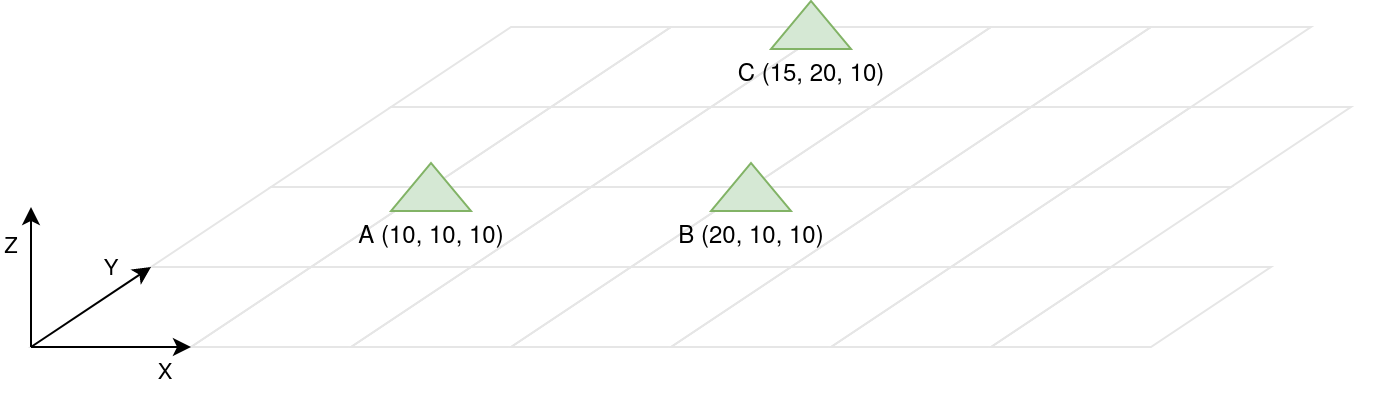
\includegraphics[width=12cm]{Programmer/benchtopo1.png}
\caption{The 3 fixed points}
\label{fig:topoEx1}
\end{figure}

The points are instances of the \texttt{cTopoPoint} class that
derives from \texttt{cObjWithUnkowns}, hence it has no copy constructor and
the points have to be added as pointers to \texttt{cTopoComp::allPts()}.

\begin{lstlisting}
  //create fixed points
  allPts.push_back(new cTopoPoint("ptA", cPt3dr(10,10,10), false));
  allPts.push_back(new cTopoPoint("ptB", cPt3dr(20,10,10), false));
  allPts.push_back(new cTopoPoint("ptC", cPt3dr(15,20,10), false));
  auto ptA = allPts[0];
  auto ptB = allPts[1];
  auto ptC = allPts[2];
\end{lstlisting}

At this point, there are no unknowns and no observations.


\subsubsection{Step 2}

A fourth point ($D$), this time not fixed, is initialized above the $ABC$ triangle.
Distances from $A$, $B$ and $C$ to $D$
are measured. For redondancy and error evaluation, the distance from $C$ to $D$ is measured twice
with different values (Fig. \ref{fig:topoEx2}).

\begin{figure}[!h]
\centering
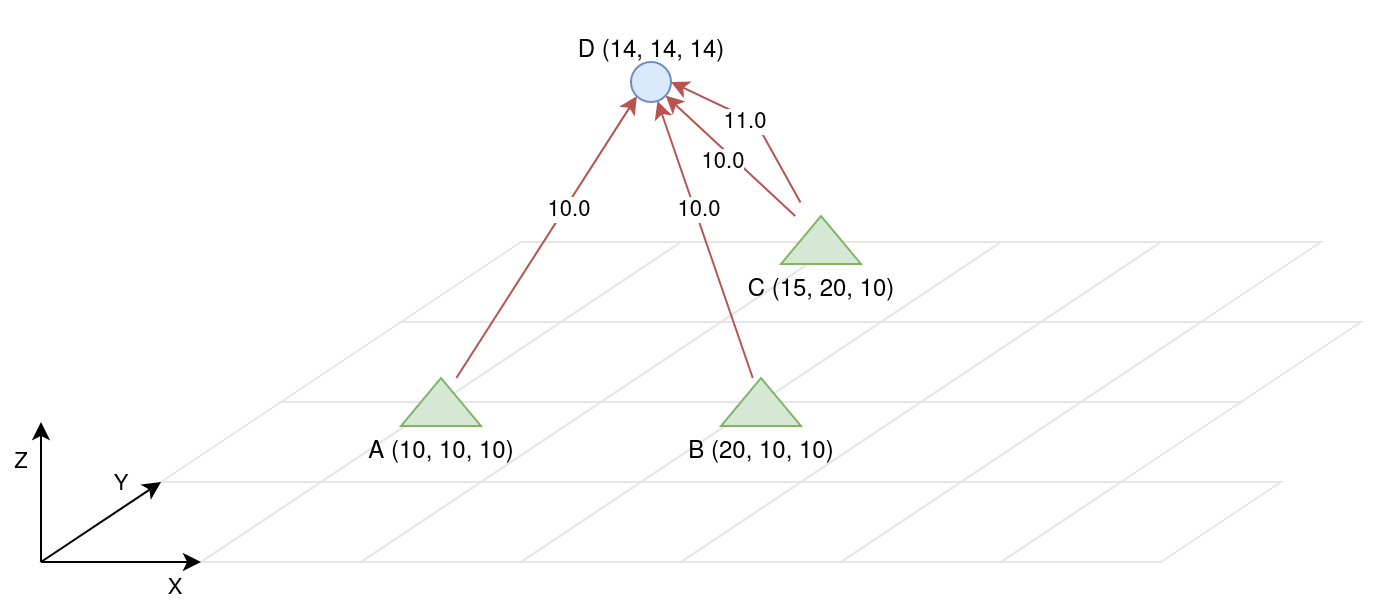
\includegraphics[width=12cm]{Programmer/benchtopo2.png}
\caption{Point $D$ is determined by measured distances}
\label{fig:topoEx2}
\end{figure}

Observations must refer to an observation set (deriving from class \texttt{cTopoObsSet})
that is used to share parameters between observations.

In the case of measured distances there is no parameter, therefore the observation set will be 
a \texttt{cTopoObsSetSimple}. Observations sets must be created with \texttt{make\_TopoObsSet} template function.

All topometric observations are instances of \texttt{cTopoObs} class.
For distances observations, \texttt{TopoObsType::dist} is given to the constructor.

\begin{lstlisting}
  //add measured dist to point D
  allObsSets.push_back(make_TopoObsSet<cTopoObsSetSimple>());
  auto obsSet1 = allObsSets[0].get();
  allPts.push_back(new cTopoPoint("ptD", cPt3dr(14,14,14), true));
  auto ptD = allPts[3];
  cTopoObs(obsSet1, TopoObsType::dist, std::vector{ptA, ptD}, {10.0});
  cTopoObs(obsSet1, TopoObsType::dist, std::vector{ptB, ptD}, {10.0});
  cTopoObs(obsSet1, TopoObsType::dist, std::vector{ptC, ptD}, {10.0});
  cTopoObs(obsSet1, TopoObsType::dist, std::vector{ptC, ptD}, {11.0});
\end{lstlisting}

The system now contains 3 unknowns ($D$ coordinates) and 4 observations
(measured distances $AD$, $BD$ and $CD$ two times).

\subsubsection{Step 3}

A second non-fixed point, $E$, is initialized inside the $ABCD$ tetrahedron,
and observations expressing that
the distances from $E$ to $A$, $B$, $C$ and $D$ are equal and unknown ($d$ in Fig. \ref{fig:topoEx3})
are added.

\begin{figure}[!h]
\centering
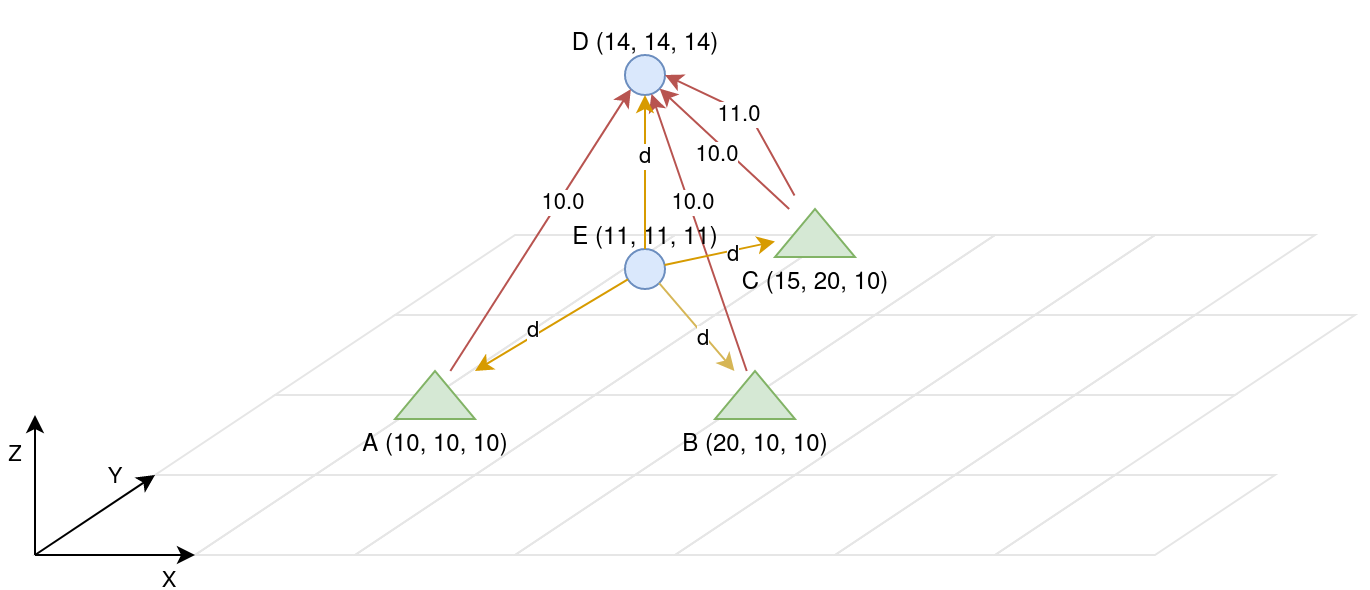
\includegraphics[width=12cm]{Programmer/benchtopo3.png}
\caption{Point $E$ determined by equal distance $d$}
\label{fig:topoEx3}
\end{figure}

A new \texttt{cTopoObsSet} must be created. The \texttt{cTopoObsSetDistParam} class
is used to create the parameter corresponding to the unknown $d$.


\begin{lstlisting}
  //add point E to an unknown common dist
  allObsSets.push_back(make_TopoObsSet<cTopoObsSetDistParam>());
  auto obsSet2 = allObsSets[1].get();
  allPts.push_back(new cTopoPoint("ptE", cPt3dr(11,11,11), true));
  auto ptE = allPts[4];
  cTopoObs(obsSet2, TopoObsType::distParam, std::vector{ptE, ptA}, {});
  cTopoObs(obsSet2, TopoObsType::distParam, std::vector{ptE, ptB}, {});
  cTopoObs(obsSet2, TopoObsType::distParam, std::vector{ptE, ptC}, {});
  cTopoObs(obsSet2, TopoObsType::distParam, std::vector{ptE, ptD}, {});
\end{lstlisting}

This adds 4 unknowns ($E$ coordinates and the unknown distance $d$) and 4 observations
($EA = EB = EC = ED = d$).


\subsection{Topometric computation}

Topometric computation system is managed by the \texttt{cTopoComp} class.
This handles the list of points and observation sets, the non-linear system
(\texttt{cResolSysNonLinear}), and a mechanism to link the observations to
the automatic derivation system.

After \texttt{cTopoComp} object creation and filling (see \ref{subsec:topoBench}),
the method \texttt{OneIteration()} is called to improve parameters estimation.

